\documentclass[11pt]{article}
% ======================================================================
%  Preambule commun - Corriges Bac Serie A (Mathematiques)
%  Style sobre : noir et blanc, sans couleurs, sans filigrane.
% ======================================================================
\usepackage[utf8]{inputenc}
\usepackage[T1]{fontenc}
\usepackage{lmodern}
\usepackage{textcomp}
\usepackage{amsmath,amssymb}
\usepackage{enumitem}
\usepackage{array}
\usepackage[a4paper,margin=2.3cm]{geometry}
\usepackage{fancyhdr}
\usepackage{tikz}
\usetikzlibrary{arrows.meta,calc,patterns}

\DeclareUnicodeCharacter{00B0}{\ensuremath{^\circ}}
\tolerance=2000
\emergencystretch=2em
\frenchspacing

\pagestyle{fancy}
\fancyhf{}
\renewcommand{\headrulewidth}{0pt}
\fancyfoot[C]{\thepage}

\newcommand{\R}{\mathbb{R}}
\newcommand{\N}{\mathbb{N}}
\newcommand{\Z}{\mathbb{Z}}
\newcommand{\vi}{\vec{\imath}}
\newcommand{\vj}{\vec{\jmath}}

\newcommand{\exo}[2]{\bigskip\noindent{\large\bfseries Exercice #1}\hfill\textit{#2}\par\nopagebreak\smallskip}
\newcommand{\partie}[1]{\medskip\noindent{\bfseries Partie #1}\par\nopagebreak\smallskip}
\newcommand{\entetesujet}[1]{\begin{center}{\Large\bfseries #1}\end{center}\vspace{0.3em}\hrule\vspace{1.1em}}

\newlist{questions}{enumerate}{1}
\setlist[questions]{label=\textbf{\arabic*.},leftmargin=1.8em,itemsep=3pt,topsep=3pt}
\newlist{sousq}{enumerate}{1}
\setlist[sousq]{label=\textbf{\alph*.},leftmargin=1.8em,itemsep=2pt,topsep=2pt}


\begin{document}

\entetecorrige{2020}{A}{Mathématiques}

\exo{1}{}
\partie{1}
\begin{questions}
  \item \begin{sousq}
    \item \textbf{Vrai}, car $28 = 7\times 4$ et $56 = 7\times 8$.
    \item \textbf{Faux}. L'équation $6x^2 - 7x + 3 = 0$ n'a pas de racine réelle : $\Delta = 7^2 - 4\times 6\times 3 = -23 < 0$.
    \item \textbf{Vrai}.
    \item \textbf{Faux}. $1 + 2 + 4 = 7$ ; 7 n'étant pas divisible par 3, 124 ne l'est pas.
  \end{sousq}
  \item \begin{sousq}
    \item PGCD de 1950 et 235 (Euclide) : $1950 = 235\times 8 + 70$ ; $235 = 70\times 3 + 25$ ; $70 = 25\times 2 + 20$ ; $25 = 20\times 1 + 5$ ; $20 = 5\times 4 + 0$. Dernier reste non nul : $\mathrm{PGCD}(1950,235) = 5$. Fraction irréductible : $\dfrac{1950}{235} = \dfrac{390}{47}$ (en divisant par 5).
    \item $8{,}297 < \dfrac{1950}{235} < 8{,}298$.
  \end{sousq}
\end{questions}

\partie{2}
\begin{questions}
  \item \underline{Conditions d'existence :} $\dfrac{2x-1}{x+4}$ existe si $x \ne -4$ ; $\dfrac{2x+1}{x-2}$ existe si $x \ne 2$. La résolution se fait sur $\R\setminus\{-4, 2\}$.
  \begin{align*}
  \frac{2x-1}{x+4} = \frac{2x+1}{x-2} &\Longleftrightarrow (2x-1)(x-2) = (2x+1)(x+4) \\
  &\Longleftrightarrow 2x^2 - 5x + 2 = 2x^2 + 9x + 4 \Longleftrightarrow -14x = 2 \Longleftrightarrow x = -\frac{1}{7}.
  \end{align*}
  D'où $S = \left\{-\dfrac{1}{7}\right\}$.
  \item \begin{sousq}
    \item $3x^2 - 2x - 1 = 0$ : discriminant réduit $\Delta' = (-1)^2 - 3\times(-1) = 4 > 0$. Solutions $x_1 = \dfrac{1-2}{3} = -\dfrac{1}{3}$ et $x_2 = \dfrac{1+2}{3} = 1$.
    \item En posant $X = e^x$, $(E') : 3e^{2x} - 2e^x - 1 = 3X^2 - 2X - 1 = 0$, d'où $X = -\dfrac{1}{3}$ (impossible, car $e^x > 0$) ou $X = 1$, soit $e^x = 1 \Leftrightarrow x = 0$. D'où $S' = \{0\}$.
  \end{sousq}
  \item \begin{sousq}
    \item De $x - 2y = -1$ : $x = 2y - 1$. Dans la 2\textsuperscript{e} équation : $7y - 2 = -2$, d'où $y = 0$ puis $x = -1$. Solution : $\{(-1\,;0)\}$.
    \item En posant $X = \ln x$, $Y = \ln y$, $(S')$ devient $\begin{cases} X - 2Y = -1 \\ 2X + 3Y = -2 \end{cases}$, d'où $X = -1$, $Y = 0$, soit $\ln x = -1$, $\ln y = 0$ : $x = \dfrac{1}{e}$, $y = 1$. Solution : $\left\{\left(\dfrac{1}{e}, 1\right)\right\}$.
  \end{sousq}
\end{questions}

\exo{2}{}
\begin{questions}
  \item \begin{sousq}
    \item $g(-1) = \dfrac{-2(-1)+2}{2(-1)+3} = 4$ : l'image de $-1$ est 4.
    \item $g$ existe si $2x + 3 \ne 0$, soit $x \ne -\dfrac{3}{2}$ : $-\dfrac{3}{2}$ n'a pas d'image.
  \end{sousq}
  \item $\lim\limits_{x\to+\infty} g(x) = \lim\limits_{x\to+\infty}\dfrac{-2x}{2x} = -1$. En $-\dfrac{3}{2}$ : $-2x+2 \to 5$ et $2x+3 \to 0$, donc $\lim\limits_{x\to-3/2^-} g = -\infty$ (car $2x+3 < 0$) et $\lim\limits_{x\to-3/2^+} g = +\infty$ (car $2x+3 > 0$).
  \item \begin{sousq}
    \item $\forall x \ne -\dfrac{3}{2}$, $g'(x) = \dfrac{-2(2x+3) - 2(-2x+2)}{(2x+3)^2} = \dfrac{-10}{(2x+3)^2}$.
    \item $(2x+3)^2 > 0$, donc $g'(x) < 0$ sur $\R\setminus\left\{-\dfrac{3}{2}\right\}$.
  \end{sousq}
  \item Tableau de variation :
  \begin{center}\renewcommand{\arraystretch}{1.4}
  \begin{tabular}{|c|ccccc|}
  \hline $x$ & $-\infty$ & & $-\frac{3}{2}$ & & $+\infty$ \\\hline
  $g'(x)$ & & $-$ & $\|$ & $-$ & \\\hline
  $g$ & $-1$ & $\searrow$ & $-\infty\ \|\ +\infty$ & $\searrow$ & $-1$ \\\hline
  \end{tabular}
  \end{center}
  \item $g(-2) = -6$ ; $g(0) = \dfrac{2}{3}$ ; $g(1) = 0$. Antécédent de 4 : $\dfrac{-2x+2}{2x+3} = 4 \Leftrightarrow -2x+2 = 8x+12 \Leftrightarrow x = -1$.
  \begin{center}\renewcommand{\arraystretch}{1.4}
  \begin{tabular}{|c|c|c|c|c|}
  \hline $x$ & $-2$ & $-1$ & $0$ & $1$ \\\hline $g(x)$ & $-6$ & $4$ & $\frac{2}{3}$ & $0$ \\\hline
  \end{tabular}
  \end{center}
  \item $g(0) = \dfrac{2}{3}$ : $(\mathcal{C})$ coupe l'axe des ordonnées en $\dfrac{2}{3}$ ; $g(1) = 0$ : elle coupe l'axe des abscisses en $x = 1$. Asymptote verticale $x = -\dfrac{3}{2}$ et asymptote horizontale $y = -1$ (en $\pm\infty$).
  \begin{center}
  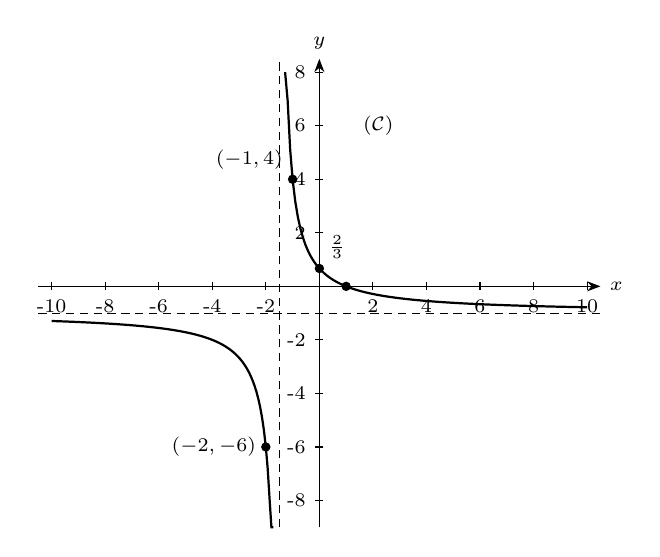
\begin{tikzpicture}[>=Stealth,scale=0.34,every node/.style={font=\scriptsize}]
    \draw[->] (-10.5,0)--(10.5,0) node[right]{$x$};
    \draw[->] (0,-9)--(0,8.5) node[above]{$y$};
    \foreach \x in {-10,-8,-6,-4,-2,2,4,6,8,10}{\draw (\x,0.15)--(\x,-0.15) node[below]{\x};}
    \foreach \y in {-8,-6,-4,-2,2,4,6,8}{\draw (0.15,\y)--(-0.15,\y) node[left]{\y};}
    \draw[densely dashed] (-1.5,-9)--(-1.5,8.5);
    \draw[densely dashed] (-10.5,-1)--(10.5,-1);
    \draw[thick] plot[domain=-1.28:10,samples=120] (\x,{min(8,(-2*\x+2)/(2*\x+3))});
    \draw[thick] plot[domain=-10:-1.72,samples=120] (\x,{max(-9,(-2*\x+2)/(2*\x+3))});
    \fill (-1,4) circle (5pt) node[above left]{$(-1,4)$};
    \fill (0,0.667) circle (5pt) node[above right]{$\frac{2}{3}$};
    \fill (1,0) circle (5pt); \fill (-2,-6) circle (5pt) node[left]{$(-2,-6)$};
    \node at (2.2,6){$(\mathcal{C})$};
  \end{tikzpicture}
  \end{center}
\end{questions}

\exo{3}{}
\begin{questions}
  \item \begin{sousq}
    \item Tableau ordonné $(T)$ :
    \begin{center}\renewcommand{\arraystretch}{1.4}
    \begin{tabular}{|c|c|c|c|c|c|c|c|c|c|c|}
    \hline $x_i$ & 5{,}5 & 5{,}6 & 5{,}6 & 5{,}8 & 6 & 6{,}2 & 6{,}4 & 6{,}8 & 7{,}1 & 7{,}2 \\
    \hline $y_i$ & 4{,}1 & 4{,}9 & 3{,}9 & 4 & 4{,}9 & 4{,}7 & 5{,}5 & 5 & 6{,}2 & 6 \\
    \hline
    \end{tabular}
    \end{center}
    \item $\overline{x}_1 = \dfrac{5{,}5 + 5{,}6 + 5{,}6 + 5{,}8 + 6}{5} = 5{,}70$ ; $\overline{y}_1 = \dfrac{4{,}1 + 4{,}9 + 3{,}9 + 4 + 4{,}9}{5} = 4{,}36$. Donc $G_1(5{,}70\,;4{,}36)$.
    \item $\overline{x}_2 = \dfrac{6{,}2 + 6{,}4 + 6{,}8 + 7{,}1 + 7{,}2}{5} = 6{,}74$ ; $\overline{y}_2 = \dfrac{4{,}7 + 5{,}5 + 5 + 6{,}2 + 6}{5} = 5{,}48$. Donc $G_2(6{,}74\,;5{,}48)$.
  \end{sousq}
  \item \begin{sousq}
    \item $y = ax + b$ passant par $G_1$, $G_2$ : $\begin{cases} 4{,}36 = 5{,}7a + b \\ 5{,}48 = 6{,}74a + b \end{cases}$. En soustrayant : $a = \dfrac{1{,}12}{1{,}04} = 1{,}077$ ; $b = 4{,}36 - 1{,}077\times 5{,}7 = -1{,}778$. D'où $y = 1{,}077x - 1{,}778$.
    \item Pour $y = 4{,}4$ : $4{,}4 = 1{,}077x - 1{,}778$, soit $x = \dfrac{6{,}178}{1{,}077} = 5{,}74$. Pour un lancer à 4,4 m du bras gauche, le lancer du bras droit est estimé à 5,74 m.
  \end{sousq}
\end{questions}

\end{document}
